\documentclass{article}
\usepackage[utf8]{inputenc}
\usepackage{url,amsmath,graphicx,amssymb,booktabs,adjustbox,subcaption,hyperref,float}
\usepackage{titlesec}
\usepackage[top=1.5cm, bottom=1.5cm, left=2.5cm, right=2.5cm]{geometry}
\usepackage{tikz}
\usetikzlibrary{positioning,shapes.multipart}

\setcounter{secnumdepth}{4}
\titleformat{\paragraph}
{\normalfont\normalsize\bfseries}{\theparagraph}{1em}{}
\titlespacing*{\paragraph}
{0pt}{3.25ex plus 1ex minus .2ex}{1.5ex plus .2ex}


\newtheorem{theorem}{Theorem}
\newtheorem{lemma}{Lemma}
\newtheorem{corollary}{Corollary}
\newtheorem{definition}{Definition}
\newtheorem{Proposition}{Proposition}

\newcommand{\Prob}{\mathbb{P}}
\newcommand{\E}{\mathbb{E}}
\newcommand{\Space}{\mathbb{S}}
\newcommand{\Var}{\text{Var}}
\newcommand{\MR}{\mathcal{R}}
\newcommand{\MT}{\mathcal{T}}

\title{MA3676 -  2018 Past Paper}
\author{1720996}

\begin{document}
\maketitle
\tableofcontents
\pagebreak

\section{Question 1}
\subsection{a}
\subsubsection{i}
\begin{equation}
    \Prob[X_{j+1}=\ldots\vert X_j=\ldots,\,X_{j-1}=\ldots,\,\ldots] = \Prob[X_{j+1}=\ldots\vert X_j=\ldots] = \frac{1}{6}     
\end{equation}
As this does not depend on any value other than previous (which even this doesn't depend on), it is a Markov chain.

\subsubsection{ii}
We have $\Prob[X=x]=\frac{1}{6}$ for all values of $x=1,\,2,\,\ldots,\,6$. Therefore,
\begin{align}
    \E[X_n] &= \frac{1}{6}\cdot 1 + \frac{1}{6}\cdot 2 + \cdots + \frac{1}{6}\cdot 6 \\
    &= \frac{1}{6}(21) \\
    &= \frac{7}{2}
\end{align}
hence 
\begin{equation}
    \E[S_n] = \frac{7}{2}n.
\end{equation}

\subsubsection{iii}
\begin{align}
    \E[X_{j+1}=\ldots\vert X_j=\ldots,\,X_{j-1}=\ldots,\,\ldots] &= \E[X_{j+1}] \\
    &\neq X_j.
\end{align}
As this doesn't hold true, $X_n$ is not a martingale.

\subsubsection{iv}
\paragraph{A}


\paragraph{B}
\begin{align}
    \E[D_{n+1}\vert \mathcal{F}_n] &= \E[D_n+Y_{n+1}\vert \mathcal{F}_n] \\
    &= D_n + \E[Y] 
\end{align}
$Y_k$ looks at the `score' obtained at each jump, so
\begin{equation}
    \E[Y] = \frac{1}{6}(+1) + \frac{1}{6}(-1) + \frac{2}{3}(0) = 0.
\end{equation}
Therefore
\begin{equation}
    \E[D_{n+1}\vert\mathcal{F}] = D_n
\end{equation}
showing that $D_n$ is a martingale.

\paragraph{C}

\subsection{b}
First, we test
\begin{align}
    G(1) &= (2-1)^{\frac{1}{2}} \\
    &= 1.
\end{align}
The first requirement is satisfied. Now, we expand $G(s)$ as follows
\begin{align}
    G(s) &= (2-s)^{\frac{1}{2}} \\
    &= \sqrt{2}\left( 1-\frac{1}{2}s \right)^{\frac{1}{2}} \\
    &= \sqrt{2}\left[ 1 - \frac{1}{2}\frac{1}{2}s - \frac{1}{2}\frac{1}{2}\frac{1}{2}\frac{1}{4}s^2 + \cdots \right] \\
    &= \sqrt{2}\left[ 1 - \frac{1}{4}s - \frac{1}{32}s^2 + \cdots\right].
\end{align}
This is enough to see that, not only does the first probability take value greater than one, we also have negative probabilities. This means that $G(s)$ \underline{\textbf{is not}} a valid generator.\\
The binomial expansion was used for the equations above.

\pagebreak
\section{Question 2}
\subsection{a}
Assigning parameters: $c=9$.\\
We have the following difference equation, where the expected time to absorption $E[\mathcal{T}_n]=T_n$
\begin{equation}
    T_n = \E[\mathcal{T}_n\vert +1]\Prob[+1] + \E[\mathcal{T}_n\vert -1]\Prob[-1].
\end{equation}
We then define the following expected values as
\begin{align}
    \E[\mathcal{T}_n\vert+1] &= 1+T_{n+1} \\
    \E[\mathcal{T}_n\vert-1] &= 1+T_{n-1} .
\end{align}
We then get the following difference equation
\begin{align}
    T_n &= \frac{1}{2}(1+T_{n+1}) + \frac{1}{2}(1+T_{n-1}) \\
    -1 &= \frac{1}{2}T_{n+1} -T_n + \frac{1}{2}T_{n-1}.
\end{align}
From this, we obtain the characteristic equation
\begin{align}
    \frac{1}{2}\lambda^2 -\lambda +\frac{1}{2} &= 0 \\
    \lambda^2 -2\lambda +1 &= 0\\
    (\lambda-1)^2 &= 0.
\end{align}
With $p=q$, we then have the general solution to the homogeneous equation 
\begin{equation}
    T_n^{(g)}=A+Bn.
\end{equation}
With a repeated root, we use the particular solution $T_n^{(p)}\alpha n^2$, remembering that $T$ is a function of $n$, giving us
\begin{equation}
    -1 = \frac{1}{2}\alpha(n+1)^2 - \alpha n^2 + \frac{1}{2}\alpha(n-1)^2. 
\end{equation}
Subbing in $n=0$ to simplify our equation, we simplify to $\alpha=-1$ and therefore a particular solution of $-n^2$. Therefore, we have the following general solution
\begin{equation}
    T_n = A+Bn-n^2.
\end{equation}
We now look at our two boundary conditions. Firstly, when we reach the the position $9N$, we know that we have reached the end point end our expected number of steps must be zero. This gives us the boundary condition
\begin{equation}
    T_{9N} = A + 9BN-(9N)^2=0
\end{equation}
Our other boundary condition exists at $n=0$. We know that, when at position $n=0$, we move $+1$ with probability $1$. This can be expressed as
\begin{align}
    \E[\mathcal{T}_n]=\E[\mathcal{T}_0\vert+1] \\
    T_0 = T_1 + 1. \label{eq:2aBoundary2}
\end{align}
We plug our general solution into~(\ref{eq:2aBoundary2}) to obtain
\begin{equation}
    A=A+B-1+1,
\end{equation}
giving us $B+0$ and therefore 
\begin{equation}
    T_n = A-n^2.
\end{equation}
We now evaluate the first boundary condition where
\begin{align}
    T_{9N} = 0 &= A - (9N)^2\\
    A &= (9N)^2.
\end{align}
We then arrive at our solution
\begin{equation}
    T_n = (9N)^2-n^2.
\end{equation}
Now we find the probability of absorption from our given starting position $S_0 = N$ with
\begin{align}
    T_N &= (9N)^2 - N^2 \\
    &= 80N^2.
\end{align}

\subsection{b}
We know by definition that $\sum_{n=0}^\infty \Prob[Z=n]=1$. Be aware that our function $C\alpha^n$ isn't valid when $n=0$, as this is defined separately as $\Prob[Z=0]=\frac{2}{3}$. Therefore, we have the following
\begin{align}
    1 &= \sum_{n=0}^\infty \Prob[Z=n] \\
    &= \frac{2}{3} + \sum_{n=1}^\infty C\alpha^n.
\end{align}
Take note of the change from $n=0$ to $n=1$. From here, we then continue to solve for $C$ in terms of $\alpha$:
\begin{align}
    \frac{1}{3} &= C\left( \sum_{n=1}^\infty \alpha^n \right) \\
    &= C\left( \sum_{n=0}^\infty \alpha^n - \sum_{n=0}^0 \alpha^n \right) \\
    &= C\left( \sum_{n=10}^\infty \alpha^n - 1\right) \\
    &= C\left( \frac{1}{1-\alpha}-1 \right) \\
    &= C\left( \frac{\alpha}{1-\alpha} \right) \\
    C &= \frac{1-\alpha}{3\alpha}.
\end{align}
Subbing in the given $\alpha = \frac{2}{3}$ gives us the result of $C=\frac{1}{6}$ and therefore the distribution rule $\Prob[Z=n]=\frac{1}{6}\left( \frac{2}{3} \right)^n$, $n\geq 1$. \\
We know that the extinction probability $\xi$ satisfies 
\begin{equation}
    G_{W_n}(\xi) = \xi
\end{equation}
So our first job is to define our generating function for some parameter $s$. The formula for a generating function $G(s)$ is as follows
\begin{equation}
    G(s) = s^n\sum_{n=0}^\infty \Prob[Z=n].
\end{equation}
We then use our values to proceed as
\begin{align}
    G(s) &= s^n\left( \sum_{n=1}^\infty \frac{1}{6}\left( \frac{2}{3} \right)^n + \frac{2}{3}\right) \\
    &= \frac{1}{6}\sum_{k=1}^\infty s^n\left( \frac{2}{3} \right)^n + s^0\frac{2}{3} \\
    &= \frac{1}{6}\sum_{k=1}^\infty \left( \frac{2s}{3} \right)^n + \frac{2}{3} \\
    &= \frac{1}{6}\left[ \sum_{k=0}^\infty \left( \frac{2s}{3} \right)^n -1 \right] + \frac{2}{3} \\
    &= \frac{1}{6}\left[ \frac{1}{1-\frac{2s}{3}} \right] + \frac{2}{3} - \frac{1}{6} \\
    &= \frac{1}{6}\left[ \frac{3}{3-2s} \right] + \frac{1}{2}.\\
\end{align}
At this point we can sub in $s=\xi$ and solve.
\begin{align}
    G(\xi) = \frac{1}{6}\left[ \frac{3}{3-2\xi} \right] + \frac{1}{2} &= \xi \\
    \frac{4-2\xi}{6-4\xi} &= \xi \\
    4-2\xi &= \xi(6-4\xi) \\
    4\xi^2-8\xi+4 &= 0 \\
    (\xi-1)(4\xi-4) &= 0
\end{align}
giving us a repeated root at $\xi=+1$. This means that our probability of extinction is certain.

\pagebreak
\section{Question 3}
\subsection{a}
\subsubsection{i}
By definition, we only need to look at the most recent state value in order to determine the following step. Therefore, the only value we nee to be aware of here is that $X_7=3$. This means that at step $7$, we are in state $3$ with probability $= 1$ as this information is definite. In order to calculate our state probabilities at $X_8$, we calculate
\begin{align}
    \mathbf{\pi}(8) &= \mathbf{\pi}(7)\mathbf{p} \\ 
    &= \begin{pmatrix} 0 & 0 & 1 & 0 & 0 & 0 \end{pmatrix}\begin{pmatrix}
        \frac{1}{2} & 0 & 0 & 0 & \frac{1}{2} & 0 \\
        0 & 0 & \frac{1}{2} & \frac{1}{2} & 0 & 0 \\
        0 & \frac{1}{3} & \frac{1}{3} & 0 & 0 & \frac{1}{3} \\
        1 & 0 & 0 & 0 & 0 & 0 \\
        \frac{1}{2} & 0 & 0 & \frac{1}{2} & 0 & 0 \\
        0 & 0 & 0 & 0 & 0 & 1
    \end{pmatrix} \\
    &= \begin{pmatrix} 0 & \frac{1}{3} & \frac{1}{3} & 0 & 0 & \frac{1}{3} \end{pmatrix}.
\end{align}
By looking at the third element of our state vector, we see that $\Prob[X_8=3] = \frac{1}{3}$. 

\subsubsection{ii}
\begin{figure}[H]
    \centering
    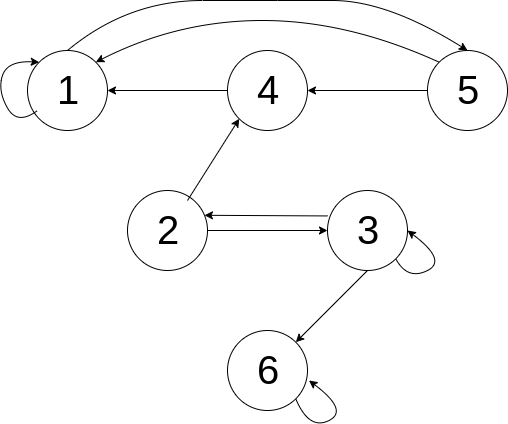
\includegraphics[scale=0.3]{diagram2020.png}
    \label{fig:3aii}
\end{figure}
We can see here that $\{1,\,4,\,5\}$ form a closed set of ergodic states and $6$ is an absorbing state. $2$ and $3$ are both transient.\\
We then restructure our state-space from $(1\,2\,3\,4\,5\,6)$ to $(1\,4\,5\,6\,2\,3)$. This in turn gives us
\begin{equation}
    \mathbf{p} = \begin{pmatrix}
        \frac{1}{2} & 0 & \frac{1}{2} & 0 & 0 & 0 \\
        1 & 0 & 0 & 0 & 0 & 0 \\
        \frac{1}{2} & \frac{1}{2} & 0 & 0 & 0 & 0 \\
        0 & 0 & 0 & 1 & 0 & 0 \\
        0 & \frac{1}{2} & 0 & 0 & 0 & \frac{1}{2} \\
        0 & 0 & 0 & \frac{1}{3} & \frac{1}{3} & \frac{1}{3}
    \end{pmatrix}.
\end{equation}
From here, it's easy enough to establish $PQR$, such that
\begin{equation}
    \mathbf{P} = \begin{pmatrix}
        \frac{1}{2} & 0 & \frac{1}{2} & 0 \\
        1 & 0 & 0 & 0 \\
        \frac{1}{2} & \frac{1}{2} & 0 & 0 \\
        0 & 0 & 0 & 1
    \end{pmatrix},
\end{equation}
\begin{equation}
    \mathbf{Q} = \begin{pmatrix}
        0 & \frac{1}{2} \\ \frac{1}{3} & \frac{1}{3}
    \end{pmatrix},
\end{equation}
\begin{equation}
    \mathbf{R} = \begin{pmatrix}
        0 & \frac{1}{2} & 0 & 0 \\
        0 & 0 & 0 & \frac{1}{3}
    \end{pmatrix}.
\end{equation}

\subsubsection{iii}
The probability is $0$ as $2$ is a transient state.

\subsubsection{iv}
The probability is $0$ as $3$ is a transient state.

\subsubsection{v}
As $5$ and $1$ are in the same closed set, we just need to find the equilibrial state of the relevant matrix for this closed set. This is found by
\begin{equation}
    \begin{pmatrix}
        \pi_1 & \pi_4 & \pi_5
    \end{pmatrix} = \begin{pmatrix}
        \pi_1 & \pi_4 & \pi_5
    \end{pmatrix}\begin{pmatrix}
        \frac{1}{2} & 0 & \frac{1}{2} \\
        1 & 0 & 0 \\
        \frac{1}{2} & \frac{1}{2} & 0
    \end{pmatrix}.
\end{equation}
From this, we obtain the following system of equations
\begin{align}
    \pi_1 &= \frac{1}{2}\pi_1 + \pi_4 + \frac{1}{2}\pi_5, \\
    \pi_4 &= \frac{1}{2}\pi_5,\\ 
    \pi_5 &= \frac{1}{2}\pi_1.
\end{align}
We use the latter two to get our stable vector in the form
\begin{equation}
    \boldsymbol{\pi} = \begin{pmatrix}
        2\pi_5 & \frac{1}{2}\pi_5 & \pi_5
    \end{pmatrix}.
\end{equation}
We know that these must sum to one so
\begin{align}
    2\pi_5 + \frac{1}{2}\pi_5 + \pi_5 &= 1 \\
    \pi_5 &= \frac{2}{7}.
\end{align}
We can then finalise our steady state as 
\begin{equation}
    \boldsymbol{\pi} = \begin{pmatrix}
        \frac{4}{7} & \frac{1}{7} & \frac{2}{7}
    \end{pmatrix}.
\end{equation}
Therefore, our final probability is the steady state probability of $X=1$ which is $\frac{4}{7}$ given that we start from within this closed set (which we did, state $5$).

\subsubsection{vi}
The probability to get absorbed in each of the closed sets is given by the elements of 
\begin{equation}
    \mathbf{\tilde{V}} = (\mathbb{I}-\mathbf{Q})^{-1}\mathbf{\tilde{R}}
\end{equation}
where 
\begin{equation}
    \mathbf{\tilde{R}} = \begin{pmatrix}
        \frac{1}{2} & 0 \\ 0 & \frac{1}{3}
    \end{pmatrix}.
\end{equation}
This gives us the following
\begin{align}
    \mathbf{\tilde{R}} &= \left( \begin{pmatrix}
        1 & 0 \\ 0 & 1
    \end{pmatrix}-\begin{pmatrix}
        0 & \frac{1}{2} \\ \frac{1}{3} & \frac{1}{3}
    \end{pmatrix} \right)^{-1}\begin{pmatrix}
        \frac{1}{2} & 0 \\ 0 & \frac{1}{3}
    \end{pmatrix}.\\
    &=  \begin{pmatrix}
        1 & -\frac{1}{2} \\ -\frac{1}{3} & \frac{2}{3}
    \end{pmatrix}^{-1}\begin{pmatrix}
        \frac{1}{2} & 0 \\ 0 & \frac{1}{3}
    \end{pmatrix}.\\
    &= 2\begin{pmatrix}
        \frac{2}{3} & \frac{1}{2} \\ \frac{1}{3} & 1
    \end{pmatrix}\begin{pmatrix}
        \frac{1}{2} & 0 \\ 0 & \frac{1}{3}
    \end{pmatrix}.\\
    &= \begin{pmatrix}
        \frac{2}{3} & \frac{1}{3} \\ \frac{1}{3} & \frac{2}{3}
    \end{pmatrix}.
\end{align}
From this, we can determine that the probability of transition from state $3$ to the closed set containing state $4$ is $\frac{1}{3}$. We then multiply this by the stable state distribution value for state $4$ found in the last question to give us $\frac{1}{3}\times\frac{1}{7}=\frac{1}{21}$.

\subsection{b}
We know one $\lambda$ value is $\frac{-1+i\sqrt{3}}{2} = e^{i2\pi/3}$, and the general formula for a periodic matrix is given as
\begin{equation}
    \lambda_k = e^{2i\pi k/d}
\end{equation}
where $d$ is the periodicity and $k=0,\,1,\ldots,\,d-1$. Therefore we can see that $k=1$ and $d=3$. This gives the other two values for this periodic set of states
\begin{align}
    \lambda_2 &= e^{4i\pi/3} = \frac{-1-i\sqrt{3}}{2},\\
    \lambda_0 &= e^0 = 1.
\end{align}
Looking at the matrix $\mathbf{p}$ we can see that state $2$ is absorbing, so we can fill in the rest of this line with $0$s and also add another $\lambda=1$ to our list. As state $3$ is clearly not one of the periodic state, we deduce that the three periodic states must be $1,4$ and $5$. We cannot tell what order these go in, so any order should suffice. Finally, state $3$ is transient and so other than filling in the row by adding the only possible value of $\frac{1}{2}$ to the line, all we know is it's eigenvalue has a magnitude strictly less than 1.
This leaves us with
\begin{equation}
    \mathbf{p}=\begin{pmatrix}
        0 & 0 & 0 & 1 & 0 \\
        0 & 1 & 0 & 0 & 0 \\
        \frac{1}{2} & \frac{1}{2} & 0 & 0 & 0 \\
        0 & 0 & 0 & 0 & 1 \\
        1 & 0 & 0 & 0 & 0
    \end{pmatrix}
\end{equation}
and the eigenvalues $\{\frac{-1+i\sqrt{3}}{2},\,1,\,r,\,\frac{-1-i\sqrt{3}}{2},\,1 \}$ where $\vert r\vert<1$.

\pagebreak
\section{Question 4}
\subsection{a}
Assigning parameters: $a = 13$, $b=1$, $c=2$, $d=9$. Therefore
\begin{align}
    r_A &= 1\% \\
    r_B &= 1\% \\
    r_C &= 2\% \\
    r_D &= 9\%. 
\end{align}

\subsubsection{i}
Our transition matrix looks like the following:
\begin{equation}
    \mathbf{p} = \begin{pmatrix}
        \frac{3}{4} & \frac{1}{4} & 0 & 0 \\
        \frac{1}{2} & \frac{1}{4} & \frac{1}{4} & 0 \\
        \frac{1}{4} & 0 & \frac{1}{4} & \frac{1}{2} \\
        \frac{3}{4} & 0 & 0 & \frac{1}{4}
    \end{pmatrix}.
\end{equation}

\subsubsection{ii}
First, we must find the steady-state vector for the transition matrix using $\boldsymbol{\pi}\mathbf{p} = \boldsymbol{\pi}$.
\begin{equation}
    \begin{pmatrix}
        \pi_A & \pi_B & \pi_C & \pi_D
    \end{pmatrix} = \begin{pmatrix}
        \pi_A & \pi_B & \pi_C & \pi_D
    \end{pmatrix}\begin{pmatrix}
        \frac{3}{4} & \frac{1}{4} & 0 & 0 \\
        \frac{1}{2} & \frac{1}{4} & \frac{1}{4} & 0 \\
        \frac{1}{4} & 0 & \frac{1}{4} & \frac{1}{2} \\
        \frac{3}{4} & 0 & 0 & \frac{1}{4}
    \end{pmatrix}.
\end{equation}
This in turn gives us the following system of equations (ignoring $\pi_A=\ldots$ as this is instead replaced by the summing to $1$, as the previous question did.)
\begin{align}
    \pi_B &= \frac{1}{4}\pi_A + \frac{1}{4}\pi_B, \\
    \pi_C &= \frac{1}{4}\pi_B + \frac{1}{4}\pi_C, \\
    \pi_D &= \frac{1}{2}\pi_C + \frac{1}{4}\pi_D.
\end{align}
Solving these in terms of $\pi_A$ gives us the following steady-state vector
\begin{equation}
    \boldsymbol{\pi} = \begin{pmatrix}
        \pi_A & \frac{1}{3}\pi_a & \frac{1}{9}\pi_A & \frac{2}{27}\pi_A
    \end{pmatrix}.
\end{equation}
Remembering that these must sum to $1$, we can solve for $\pi_A$ and get our final steady state.
\begin{align}
    \pi_A\left( \frac{27 + 9 + 3 + 2}{27} \right) &= 1 \\
    \pi_A &= \frac{27}{41}. 
\end{align}
This leaves us with
\begin{equation}
    \boldsymbol{\pi} = \begin{pmatrix}
        \frac{27}{41} & \frac{9}{41} & \frac{3}{41} & \frac{2}{41}
    \end{pmatrix}.
\end{equation}
Remaining to be finished later.

\subsection{b}





\end{document}
